\chapter{Simulation}

In the initial stages of the project, hardware procurement had significant lead times, with testing and integration adding further delays. Thus, a simulation environment was developed in PyBullet so that control logic could be validated in the meantime. This enabled rapid iteration of the finite state machine logic without risking hardware damage, and visualisation of different camera perspectives and tracking behaviour before procuring --- let alone mounting --- any physical camera.

The physical world consists of a conveyor belt modelled as a static rigid body and a box which spawns with a random X position and yaw angle on the line. To model conveyor motion, the box position is reset each timestep rather than using contact forces, because physical fidelity was not the purpose of the simulation.

The gantry itself is modelled using the Unified Robot Description Format (URDF). The kinematic chain begins at a fixed world-interface link, followed by a prismatic X joint driving the bridge, a prismatic Y joint for the carriage, a prismatic Z joint for the vertical probe, a revolute yaw joint at the end-effector, and finally two prismatic finger joints. The end-effector is modelled through a gripping mechanism rather than the vacuum system used in the final hardware; however, the degrees of freedom are identical, and the simulation's purpose --- validating the finite state machine and IBVS control law --- is unaffected by the gripping mechanism. To simplify matters, the robot applies a rigid fixed constraint between the end-effector link and the box upon contact, bypassing contact force modelling entirely.

Image-based visual servoing (IBVS) was implemented and tested within the simulation using pixel data from a virtual camera attached to the gantry frame. The IBVS controller successfully converged on the target object across randomised initial positions and yaw angles, confirming the viability of the control law described in Section~\ref{sec:classical_pipeline} prior to deployment on physical hardware.

\begin{figure}[H]
    \centering
    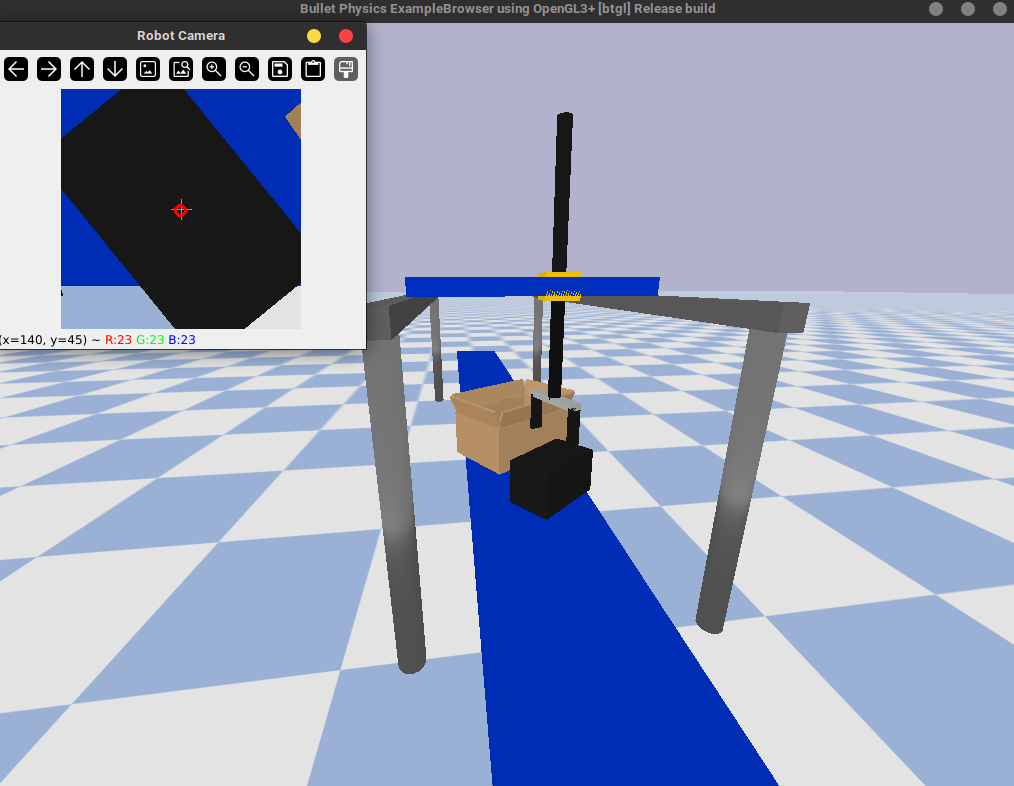
\includegraphics[width=0.9\linewidth]{figures/ibvs.png}
    \caption{IBVS in simulation. The inset shows the virtual camera view with the detected target; the main view shows the gantry converging on the box.}
    \label{fig:ibvs_sim}
\end{figure}